\documentclass[10pt, aspectratio=169]{beamer}

% --- Configuración del Tema ---
\usetheme{metropolis}
\usecolortheme{owl} 
\usepackage[spanish]{babel}
\usepackage[utf8]{inputenc}
\usepackage{amsfonts, amsmath, amssymb, amsthm}
\usepackage{graphicx}
\usepackage{tikz}

% --- Entornos Matemáticos ---
\newtheorem{definicion}{Definición}

% --- Colores Personalizados ---
\definecolor{diagonalred}{RGB}{140, 20, 40}

\title{Los Límites de la Razón}
\subtitle{Sesión 6: La Ilusión de la Inteligencia}
\author{Rosh Guadiana}
\date{Verano 2026}

\begin{document}

\maketitle

% ==========================================
% ACTO 1: EL DESCENSO A LA MATERIA
% ==========================================

\begin{frame}{El Arquitecto del Pensamiento Abstracto}
    \begin{columns}
        \begin{column}{0.4\textwidth}
            \begin{center}
                \includegraphics[height=0.65\textheight]{../../assets/George-Boole.jpg} \\
                \vspace{0.2cm}
                \textbf{George Boole} \\
                \small (1815 -- 1864)
            \end{center}
        \end{column}
        \begin{column}{0.6\textwidth}
            \vspace{0.5cm}
            \Large \textbf{La Sintaxis en el Vacío}
            
            \vspace{0.4cm}
            \normalsize
            Boole inventó su álgebra sintáctica creyendo que estaba modelando \textit{las leyes del pensamiento humano}. Esa sintaxis permaneció abstracta, inmaterial e incorpórea durante casi un siglo.
        \end{column}
    \end{columns}
\end{frame}

\begin{frame}{El Ingeniero de la Realidad}
    \begin{columns}
        \begin{column}{0.4\textwidth}
            \begin{center}
                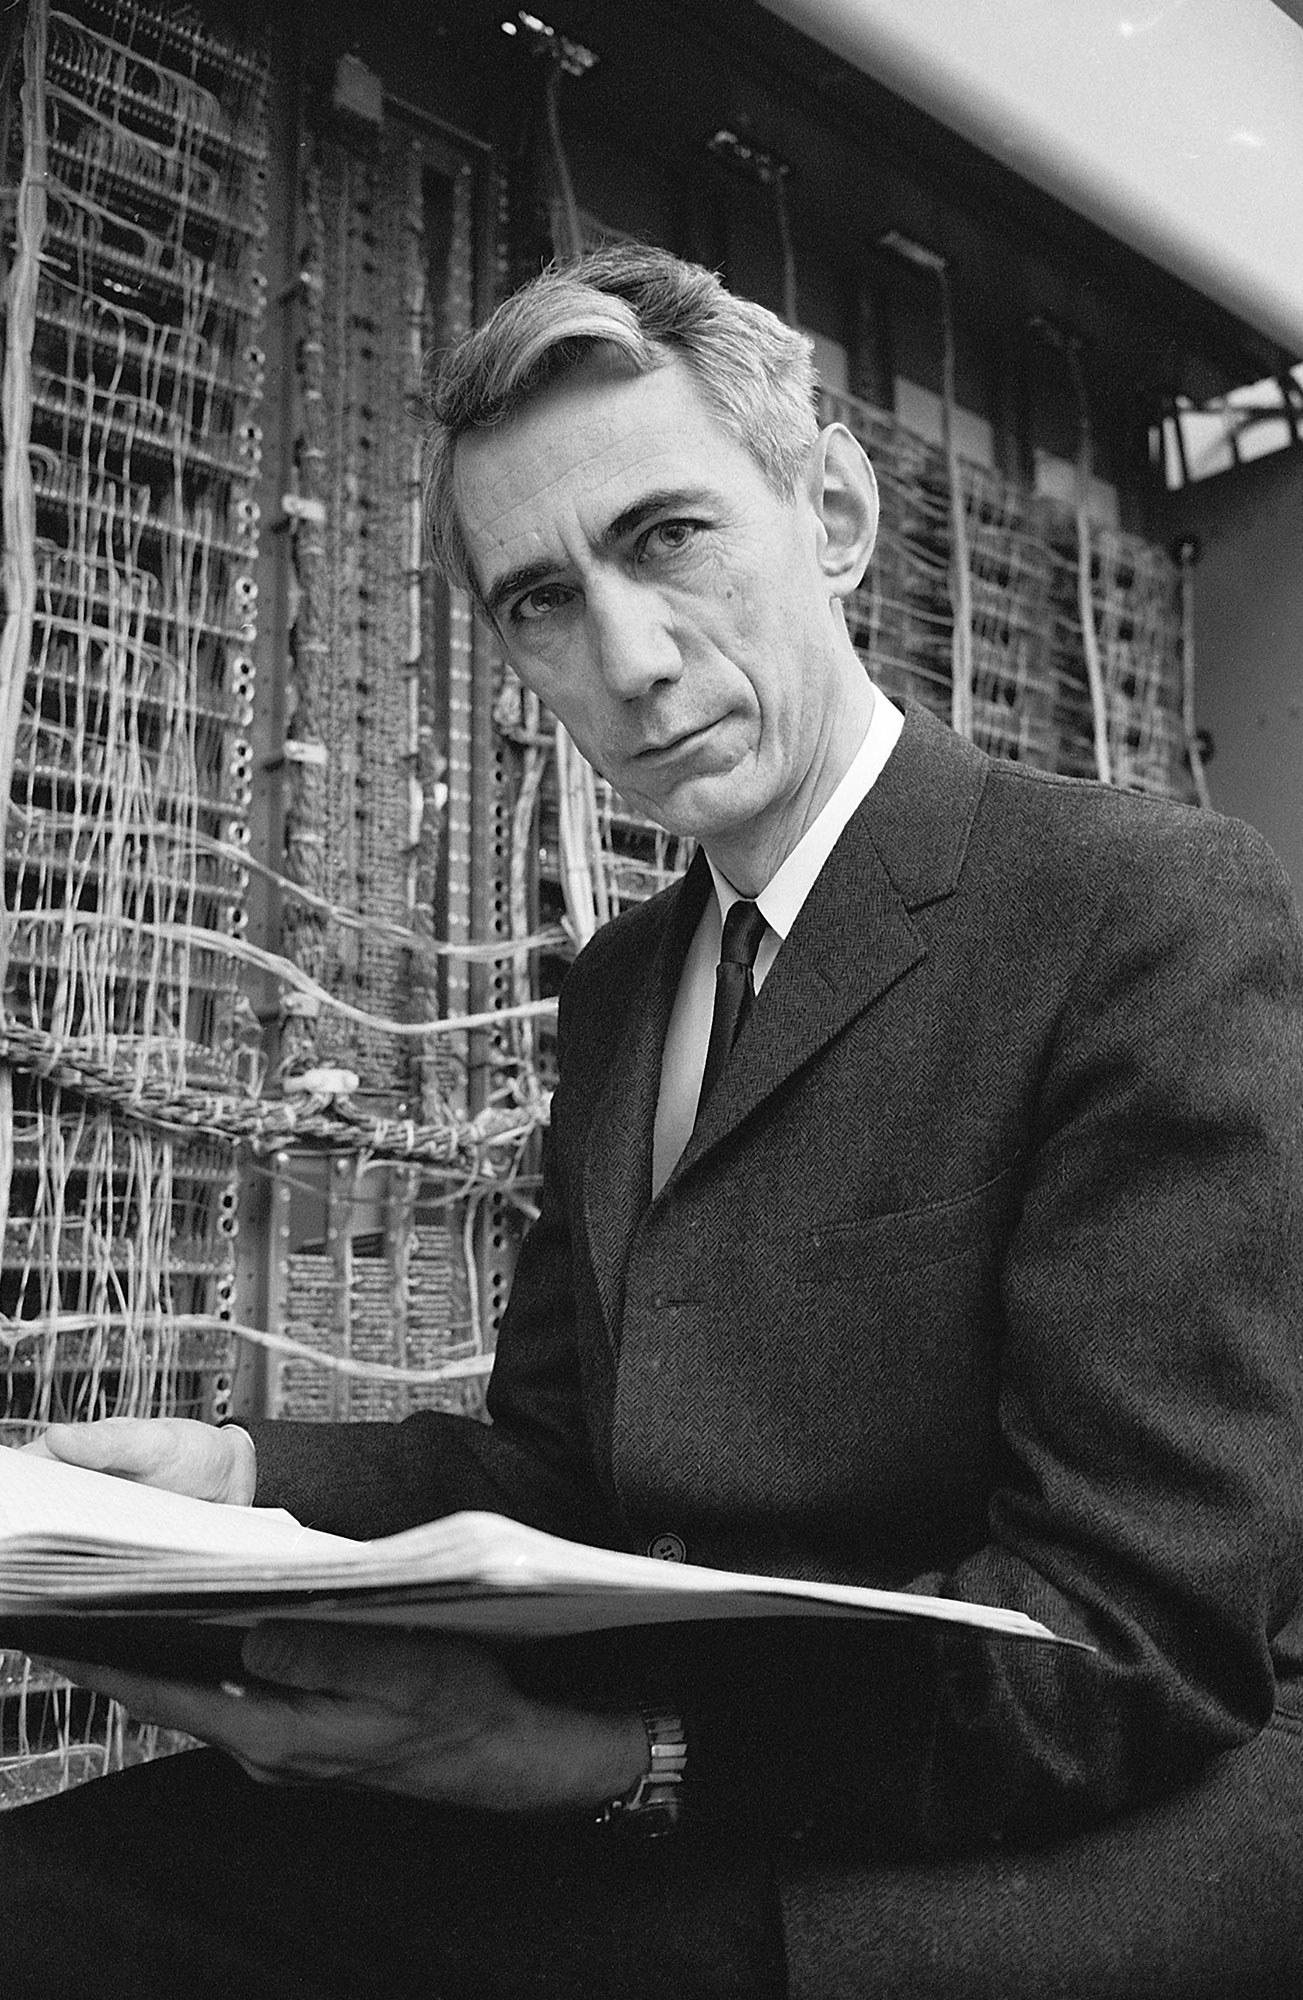
\includegraphics[height=0.65\textheight]{../../assets/Claude-Shannon.jpg} \\
                \vspace{0.2cm}
                \textbf{Claude Shannon} \\
                \small (1916 -- 2001)
            \end{center}
        \end{column}
        \begin{column}{0.6\textwidth}
            \vspace{0.5cm}
            \Large \textbf{El Isomorfismo Físico (1938)}
            
            \vspace{0.4cm}
            \normalsize
            En su tesis de maestría en el MIT, Shannon demostró matemáticamente que los circuitos de relés electromecánicos operan bajo los mismos postulados axiomáticos que el álgebra de Boole.
            
            \vspace{0.4cm}
            \alert{\textbf{La lógica acababa de convertirse en electricidad.}}
        \end{column}
    \end{columns}
\end{frame}

\begin{frame}{La Materialización de la Sintaxis}
    \begin{center}
        \textbf{Circuitos de Conmutación Analizados con Álgebra Booleana}
        
        \vspace{0.6cm}
        \begin{tikzpicture}[scale=1.2, thick]
            % Circuito en Serie (AND)
            \node at (2, 2.5) {\alert{\textbf{Operación AND ($A \land B$)}}};
            \draw (0,1.5) -- (1,1.5);
            \draw[fill=white] (1,1.5) circle (0.05);
            \draw (1,1.9) -- (2,1.5); 
            \draw[fill=white] (2,1.5) circle (0.05);
            \draw (2,1.5) -- (3,1.5);
            \draw[fill=white] (3,1.5) circle (0.05);
            \draw (3,1.9) -- (4,1.5); 
            \draw[fill=white] (4,1.5) circle (0.05);
            \draw (4,1.5) -- (5,1.5);
            \node at (1.5, 2.1) {$A$};
            \node at (3.5, 2.1) {$B$};

            % Circuito en Paralelo (OR)
            \begin{scope}[shift={(6, 0)}]
                \node at (2, 2.5) {\alert{\textbf{Operación OR ($A \lor B$)}}};
                \draw (0,1.5) -- (0.5,1.5) -- (0.5,2) -- (1,2);
                \draw[fill=white] (1,2) circle (0.05);
                \draw (1,2.4) -- (2,2); 
                \draw[fill=white] (2,2) circle (0.05);
                \draw (2,2) -- (3.5,2) -- (3.5,1.5) -- (4,1.5);
                
                \draw (0.5,1.5) -- (0.5,1) -- (1,1);
                \draw[fill=white] (1,1) circle (0.05);
                \draw (1,1.4) -- (2,1); 
                \draw[fill=white] (2,1) circle (0.05);
                \draw (2,1) -- (3.5,1);
                
                \node at (1.5, 2.6) {$A$};
                \node at (1.5, 1.6) {$B$};
            \end{scope}
        \end{tikzpicture}
    \end{center}
\end{frame}

% ==========================================
% ACTO 2: ENGRANAJES Y AUTÓMATAS
% ==========================================

\begin{frame}{El Engranaje Lógico}
    \vspace{0.4cm}
    \Large \textbf{La máquina sin semántica}
    
    \vspace{0.4cm}
    \normalsize
    Antes de modelar la vida, debemos aislar su motor físico. Imaginen un reloj mecánico: no "sabe" qué hora es y carece de consciencia del tiempo. 
    
    \vspace{0.6cm}
    Solo posee \textbf{estados físicos} (la posición de los engranajes) y una \textbf{regla de transición inquebrantable} (la acción del péndulo). Es una máquina ciega de estímulo y reacción: \textit{El Autómata}.
\end{frame}

\begin{frame}{Definición Formal: Autómata Finito (FSA)}
    \begin{definicion}[Autómata Finito]
        Una máquina de estados finitos es una construcción matemática rigurosa definida por la 5-tupla:
        $$M = \langle Q, \Sigma, \delta, q_0, F \rangle$$
    \end{definicion}
    
    \vspace{0.2cm}
    \textbf{Donde:}
    \begin{itemize}
        \setlength\itemsep{0.2cm}
        \item $Q$: Conjunto finito de \textbf{estados}.
        \item $\Sigma$: Alfabeto de \textbf{entradas} (estímulos).
        \item $\delta$: Función de \textbf{transición} inmutable, $\delta: Q \times \Sigma \to Q$.
        \item $q_0 \in Q$: Estado inicial.
        \item $F \subseteq Q$: Conjunto de estados finales o de aceptación.
    \end{itemize}
\end{frame}

\begin{frame}{Mecánica del Autómata: El Torniquete}
    \begin{center}
        \textbf{Demostración: } $Q = \{B, D\}$, $\quad \Sigma = \{\text{Moneda}, \text{Empujar}\}$
        
        \vspace{0.8cm}
        \begin{tikzpicture}[scale=1.2, thick, >=stealth]
            % Estados
            \node[draw=white, circle, minimum size=1.5cm, align=center] (B) at (0,0) {$B$ \\ (Bloqueado)};
            \node[draw=white, circle, minimum size=1.5cm, align=center] (D) at (5,0) {$D$ \\ (Desbloqueado)};
            
            % Transiciones
            \draw[->] (B) to[bend left=20] node[midway, above] {\alert{Moneda}} (D);
            \draw[->] (D) to[bend left=20] node[midway, below] {\alert{Empujar}} (B);
            
            % Bucle
            \draw[->] (B) arc (20:340:0.6) node[midway, left=0.1cm] {\alert{Empujar}};
        \end{tikzpicture}
        
        \vspace{0.8cm}
        \normalsize
        \textbf{Ecuaciones de Transición ($\delta$):} \\
        $\delta(B, \text{Moneda}) = D \quad \mid \quad \delta(D, \text{Empujar}) = B \quad \mid \quad \delta(B, \text{Empujar}) = B$
    \end{center}
\end{frame}

\begin{frame}{El Proyecto Los Álamos: La Autorreplicación}
    \begin{columns}
        \begin{column}{0.3\textwidth}
            \begin{center}
                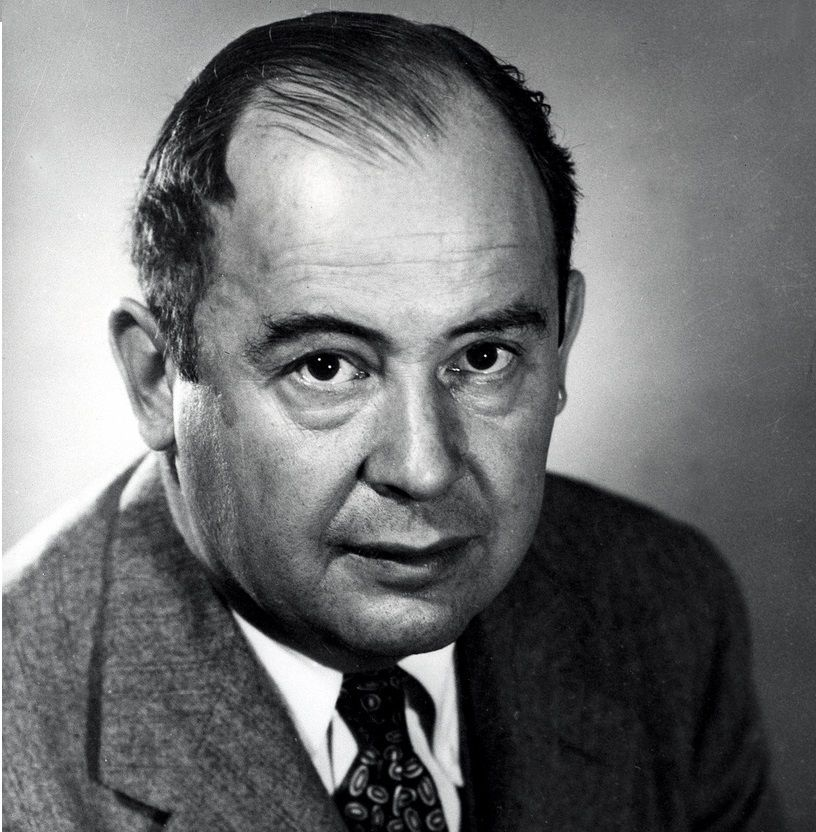
\includegraphics[height=0.4\textheight]{../../assets/John-von-Neumann.jpg} \\
                \vspace{0.1cm}
                \footnotesize \textbf{John von Neumann} \\ (1903 -- 1957)
                
                \vspace{0.3cm}
                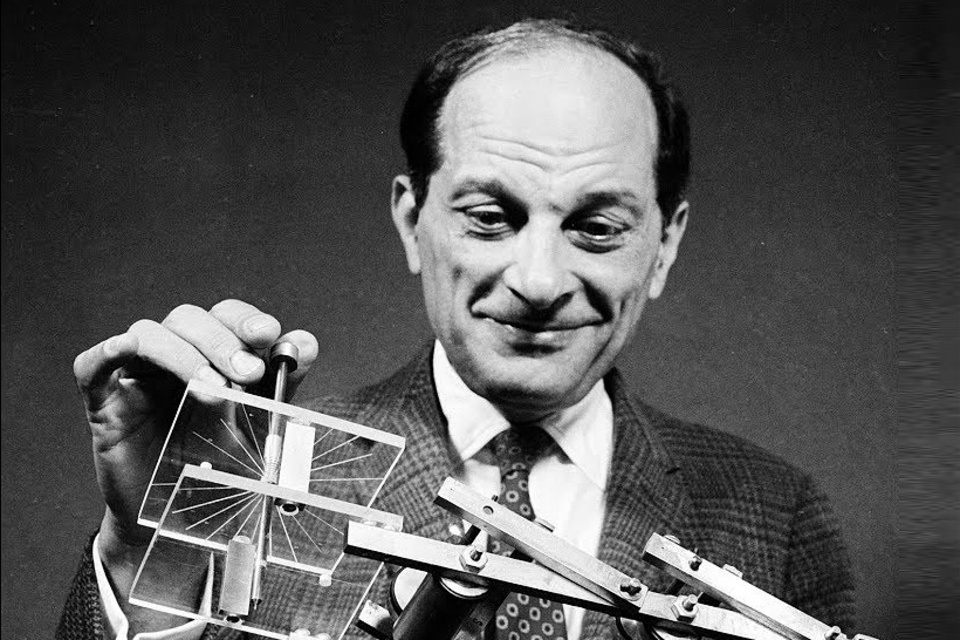
\includegraphics[height=0.4\textheight]{../../assets/Stanislaw-Ulam.jpg} \\
                \vspace{0.1cm}
                \footnotesize \textbf{Stanislaw Ulam} \\ (1909 -- 1984)
            \end{center}
        \end{column}
        \begin{column}{0.7\textwidth}
            \vspace{0.5cm}
            \Large \textbf{Los Primeros Autómatas Celulares}
            
            \vspace{0.4cm}
            \normalsize
            Pasamos de un torniquete a una cuadrícula infinita. Buscaban entender cómo la vida se replica matemáticamente usando complejos sistemas de 29 estados.
            
            \vspace{0.4cm}
            \alert{\textbf{El dogma mecanicista:}} \\
            Von Neumann asumía erróneamente que, para generar complejidad, se requería obligatoriamente una \textit{unidad de control central}.
        \end{column}
    \end{columns}
\end{frame}

\begin{frame}{El Destructor del Control Central}
    \begin{columns}
        \begin{column}{0.4\textwidth}
            \begin{center}
                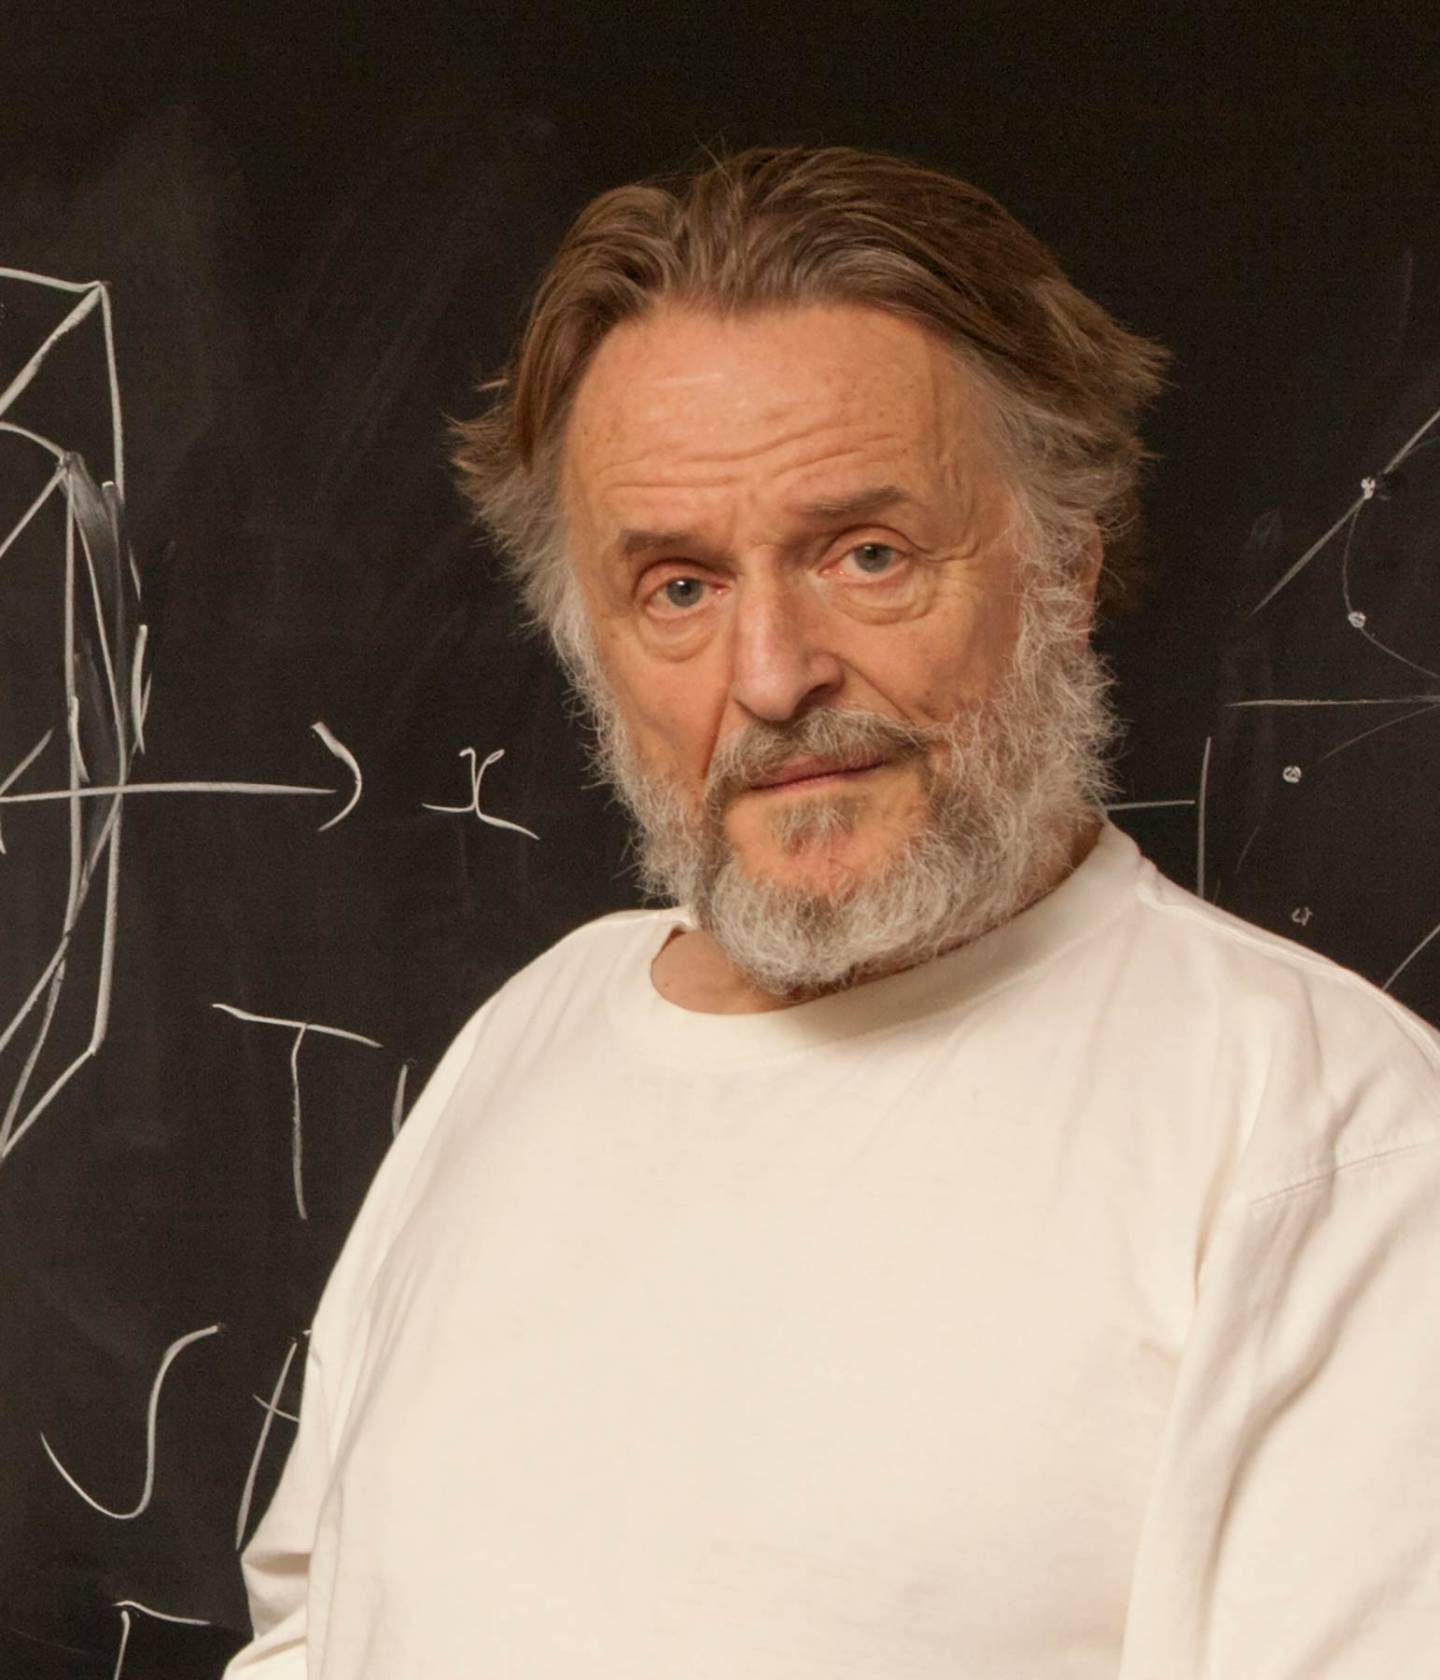
\includegraphics[height=0.65\textheight]{../../assets/John-Conway.jpg} \\
                \vspace{0.2cm}
                \textbf{John Conway} \\
                \small (1937 -- 2020)
            \end{center}
        \end{column}
        \begin{column}{0.6\textwidth}
            \vspace{0.5cm}
            \Large \textbf{El Juego de la Vida (1970)}
            
            \vspace{0.4cm}
            \normalsize
            Conway destruyó el paradigma del diseñador central. Demostró que la emergencia del caos y la complejidad absoluta surgen de la \textbf{ceguera local}. No se necesita un "cerebro" dirigiendo el sistema.
        \end{column}
    \end{columns}
\end{frame}

\begin{frame}{Reglas Atómicas de Conway}
    \vspace{0.4cm}
    \Large \textbf{El universo en tres axiomas:}
    
    \vspace{0.6cm}
    \normalsize
    \begin{itemize}
        \setlength\itemsep{0.5cm}
        \item \alert{\textbf{Supervivencia:}} Una célula viva con 2 o 3 vecinas vivas, sobrevive a la siguiente generación.
        \item \alert{\textbf{Asfixia:}} Una célula viva con más de 3 vecinas muere (sobrepoblación), o con menos de 2 muere (aislamiento).
        \item \alert{\textbf{Nacimiento:}} Una célula muerta con exactamente 3 vecinas vivas, se enciende.
    \end{itemize}
\end{frame}

\begin{frame}{La Emergencia de la Complejidad}
    \begin{center}
        \Large \textbf{Dinámica del Juego de la Vida}
        
        \vspace{0.4cm}
        % Aquí proyectarás imágenes o GIFs de Gliders, Gosper Glider Guns, etc.
        \includegraphics[height=0.6\textheight]{../../assets/conway_patterns.png}
        
        \vspace{0.4cm}
        \footnotesize \textit{Estructuras estables, osciladores y naves espaciales emergen de reglas sin consciencia global.}
    \end{center}
\end{frame}

% ==========================================
% REGLA 30 DE WOLFRAM
% ==========================================

\begin{frame}{La Regla 30: La Muerte del Arquitecto}
    \begin{columns}
        \begin{column}{0.4\textwidth}
            \vspace{0.2cm}
            \Large \textbf{El espacio de Wolfram}
            
            \vspace{0.4cm}
            \normalsize
            Stephen Wolfram decidió estudiar el caso analítico más primitivo posible:
            \begin{itemize}
                \item Una dimensión ($d=1$).
                \item Binario ($S=\{0,1\}$).
                \item Vecindario mínimo ($|N|=3$).
            \end{itemize}
        \end{column}
        \begin{column}{0.6\textwidth}
            \vspace{0.5cm}
            Dado un vecindario de 3 celdas binarias, hay $2^3 = 8$ estados vecinales posibles (desde $111$ hasta $000$).
            
            \vspace{0.4cm}
            Por permutación, existen exactamente $2^8 = \alert{\textbf{256 reglas o universos posibles}}$.
            
            \vspace{0.4cm}
            Wolfram las enumeró. Estudiaremos la número 30 (en binario: \textbf{00011110}).
        \end{column}
    \end{columns}
\end{frame}

\begin{frame}{Desglose Matemático de la Regla 30}
    \begin{center}
        \textbf{Tabla de Transición (Regla 30)}
        
        \vspace{0.4cm}
        \begin{tabular}{|c|c|c|c|c|c|c|c|c|}
            \hline
            $t$ (Vecindario) & 111 & 110 & 101 & 100 & 011 & 010 & 001 & 000 \\
            \hline
            $t+1$ (Nueva celda) & \textbf{0} & \textbf{0} & \textbf{0} & \textbf{1} & \textbf{1} & \textbf{1} & \textbf{1} & \textbf{0} \\
            \hline
        \end{tabular}
        
        \vspace{0.8cm}
        \Large \textbf{El Álgebra del Universo}
        
        \vspace{0.2cm}
        \normalsize
        En el anillo booleano, la evolución temporal se reduce a pura lógica:
        
        \vspace{0.4cm}
        \huge
        $$c_i^{t+1} = c_{i-1}^t \oplus (c_i^t \lor c_{i+1}^t)$$
    \end{center}
\end{frame}

\begin{frame}{La Iteración del Tiempo}
    \begin{center}
        \Large \textbf{Estallido desde el vacío}
        
        \vspace{0.4cm}
        \normalsize
        Iniciamos un universo muerto de ceros infinitos, con un único $1$ como chispa inicial.
        
        \vspace{0.6cm}
        \large
        $t=0$: \quad $\dots \quad 0 \quad 0 \quad 0 \quad [\mathbf{1}] \quad 0 \quad 0 \quad 0 \quad \dots$
        
        \vspace{0.4cm}
        \alert{$\delta(0,0,1)=1 \quad \delta(0,1,0)=1 \quad \delta(1,0,0)=1$}
        
        \vspace{0.4cm}
        $t=1$: \quad $\dots \quad 0 \quad 0 \quad [\mathbf{1} \quad \mathbf{1} \quad \mathbf{1}] \quad 0 \quad 0 \quad \dots$
        
        \vspace{0.4cm}
        $t=2$: \quad $\dots \quad 0 \quad \mathbf{1} \quad \mathbf{1} \quad 0 \quad 0 \quad \mathbf{1} \quad 0 \quad \dots$
        
        \vspace{0.6cm}
        \normalsize
        \textit{La asimetría de la regla XOR/OR acaba de romper el vacío.}
    \end{center}
\end{frame}

\begin{frame}{El Patrón de Wolfram}
    \begin{center}
        \Large \textbf{Irreducibilidad Computacional}
        
        \vspace{0.4cm}
        % Aquí proyectarás la imagen de la pirámide asimétrica generada por la Regla 30
        \includegraphics[height=0.6\textheight]{../../assets/rule30.png}
        
        \vspace{0.4cm}
        \footnotesize \textit{La naturaleza no necesita un código inmenso; solo iteración matemática profunda.}
    \end{center}
\end{frame}

% ==========================================
% ACTO 3: LA SINTAXIS DE LA VIDA
% ==========================================

\begin{frame}{La Gramática Botánica}
    \begin{columns}
        \begin{column}{0.4\textwidth}
            \begin{center}
                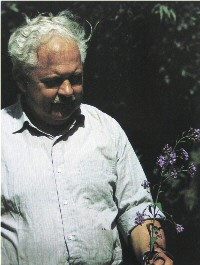
\includegraphics[height=0.65\textheight]{../../assets/Aristid-Lindenmayer.jpg} \\
                \vspace{0.2cm}
                \textbf{Aristid Lindenmayer} \\
                \small (1925 -- 1989)
            \end{center}
        \end{column}
        \begin{column}{0.6\textwidth}
            \vspace{0.5cm}
            \Large \textbf{L-Systems (1968)}
            
            \vspace{0.4cm}
            \normalsize
            Botánico húngaro que formalizó el crecimiento morfológico de las plantas no como biología orgánica, sino como una \textbf{gramática generativa puramente sintáctica}.
            
            \vspace{0.4cm}
            \alert{\textbf{Regla recursiva simple (Crecimiento fractal):}} \\
            $A \to AB$ \\
            $B \to A$
        \end{column}
    \end{columns}
\end{frame}

\begin{frame}{La Máquina de Dibujar Biología}
    \begin{columns}
        \begin{column}{0.4\textwidth}
            \begin{center}
                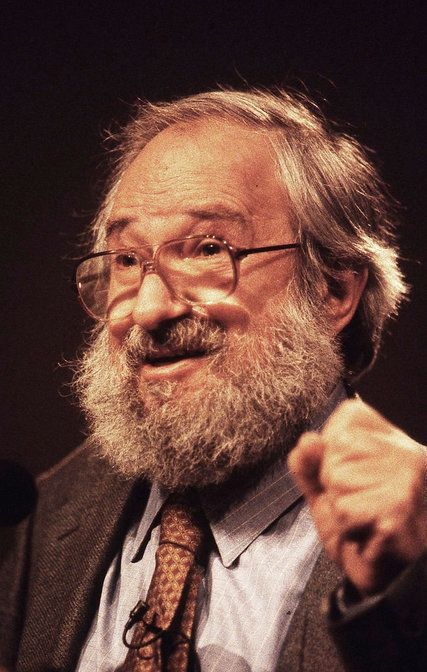
\includegraphics[height=0.65\textheight]{../../assets/Seymour-Papert.jpg} \\
                \vspace{0.2cm}
                \textbf{Seymour Papert} \\
                \small (1928 -- 2016)
            \end{center}
        \end{column}
        \begin{column}{0.6\textwidth}
            \vspace{0.5cm}
            \Large \textbf{El lenguaje Logo y la Tortuga}
            
            \vspace{0.4cm}
            \normalsize
            Pionero de la inteligencia artificial en el MIT. Al obligar a su robot virtual ("la tortuga") a ejecutar los axiomas recursivos de Lindenmayer mediante comandos ciegos de giro y avance...
            
            \vspace{0.4cm}
            \alert{\textbf{La pantalla generó ecosistemas.}}
        \end{column}
    \end{columns}
\end{frame}

\begin{frame}{Fractales Orgánicos}
    \begin{center}
        \Large \textbf{L-Systems en Acción}
        
        \vspace{0.4cm}
        % Aquí proyectarás los matorrales generados por código recursivo
        \includegraphics[height=0.6\textheight]{../../assets/lsystems_trees.png}
        
        \vspace{0.4cm}
        \footnotesize \textit{Morfología vegetal hiperrealista generada exclusivamente por sintaxis y geometría.}
    \end{center}
\end{frame}

\begin{frame}{El Cierre Filosófico: La Inteligencia Aparente}
    \vspace{0.8cm}
    \begin{center}
        \huge \textit{``No hay nadie en casa.''}
    \end{center}
    
    \vspace{0.8cm}
    \normalsize
    \alert{\textbf{El espejismo del diseñador:}} \\
    Al ver a la tortuga dibujar árboles hiperrealistas o al autómata simular vida y caos, el cerebro humano proyecta consciencia. Es una ilusión total. La máquina no "entiende" el árbol; no "comprende" la vida. 
    
    \vspace{0.6cm}
    Solo está evaluando sintaxis vacía, moviendo cargas eléctricas bajo reglas preestablecidas absolutamente ciegas.
\end{frame}

\end{document}
